\documentclass[11pt,a4paper]{article}

\usepackage[a4paper,margin=1in]{geometry}
\usepackage[T1]{fontenc}
\usepackage[utf8]{inputenc}
\usepackage{lmodern}
\usepackage{setspace}
\usepackage{hyperref}
\usepackage{xurl}
\usepackage{microtype}
\usepackage{graphicx}

\setstretch{1.0}
\urlstyle{tt}
\emergencystretch=2em

\title{Software Development Report}
\author{Brandon MacGillivray}
\date{\today}

\begin{document}

\hypersetup{pageanchor=false}
\begin{titlepage}
\centering
{\LARGE Software Development Report\par}
\vspace{1.5cm}
{\large An investigation into Lightweight Hand Pose estimation for Edge HCI\par}
\vspace{1cm}
{\large Brandon MacGillivray\par}
\vspace{0.5cm}
{\large 40321491\par}
\vfill
\end{titlepage}
\hypersetup{pageanchor=true}

\tableofcontents
\newpage

\section{Purpose, Operation and Validation}

\noindent This software is a gesture-driven interactive demo developed for live
presentation. Its purpose is to allow a demo user to explore prepared visual
outputs through direct hand interaction rather than through command-line
experiments or conventional desktop controls.

\medskip

\noindent The primary user story for this demo is: ``As a demo user, I want to
control the demo through hand gestures so that I can navigate the
showcase and inspect the prepared visual outputs without relying on a mouse or
keyboard.''

\medskip

\noindent In operation, the demo opens the ZED camera, detects one hand, and
uses the tracked hand as the main control input. Palm movement is used to drive
an on-screen cursor, while a fist gesture is interpreted as a click. Through
this interaction model, the user can move from the start page to the menu and
then select either the segmentation demonstration or the tone-mapping
demonstration.

\medskip

\noindent The software can be considered to be working correctly when it starts successfully,
detects the camera, shows stable cursor movement in response to hand motion,
registers fist gestures as intended selections, allows the user to navigate the
demonstration pages correctly, and updates the visual outputs in the expected
way.

\section{Design and Implementation}

\subsection{Significant Assumptions Made for the Design and Implementation}

This demo assumes that a working ZED camera is connected and available at runtime, that a
single hand can be tracked reliably enough for gesture-based interaction, that
the application is used in its intended portrait presentation layout, that the
required segmentation and tone-mapping assets are already present locally, and
that the application is launched from the expected working directory so that
its relative asset paths resolve correctly during execution.

\subsection{Languages, Packages, Frameworks, and Libraries Used}

The demo was implemented in Python 3.10, with PySide6 used for the
graphical user interface, MediaPipe used for hand tracking, and
\texttt{pyzed} used for interaction with the ZED camera. 
With support from OpenCV, Pillow and NumPy.

\subsection{Overall Architecture / System Design and Interfaces Between Components}

The demo was implemented as a small interactive architecture with
three main parts. First, a perception pipeline acquires frames from the ZED
camera, preprocesses them, and applies MediaPipe Hands to estimate landmarks
from which cursor position, palm width, and fist-click state are derived.
Second, a central \texttt{MainWindow} acts as the controller for the
application: it receives pose updates, maintains the active page, updates the
overlay, routes gesture-derived click events to the appropriate page logic,
and triggers timeout recovery when tracking is lost. Third, the presentation
layer is implemented as a set of pages for the start screen, menu,
segmentation demonstration, and tone-mapping demonstration, with the content
pages loading prepared visual assets from disk.

\medskip

This structure was chosen because it separates latency-sensitive vision
processing from presentation logic while still allowing both demonstrations to
share the same interaction controller. The perception pipeline is responsible
for deriving interaction state from live camera input, the controller manages
application state and gesture routing, and the presentation layer is
responsible for what the user sees. This separation reduces coupling between
different responsibilities, helps keep the interface responsive during live
use, and makes the overall flow of interaction easier to understand.

\medskip

Alternative designs were possible. For example, camera acquisition, hand
tracking, and page behaviour could have been implemented directly inside the
GUI event loop or combined within a more monolithic single-class design.
However, this approach was not chosen because it would have made the
application more tightly coupled, harder to reason about, and more likely to
become unresponsive during live interaction. The adopted design was thus
more appropriate for a demo that depended on real-time tracking and
clear separation between interaction logic and presentation behaviour.

\medskip

\begin{figure}[htbp]
\centering
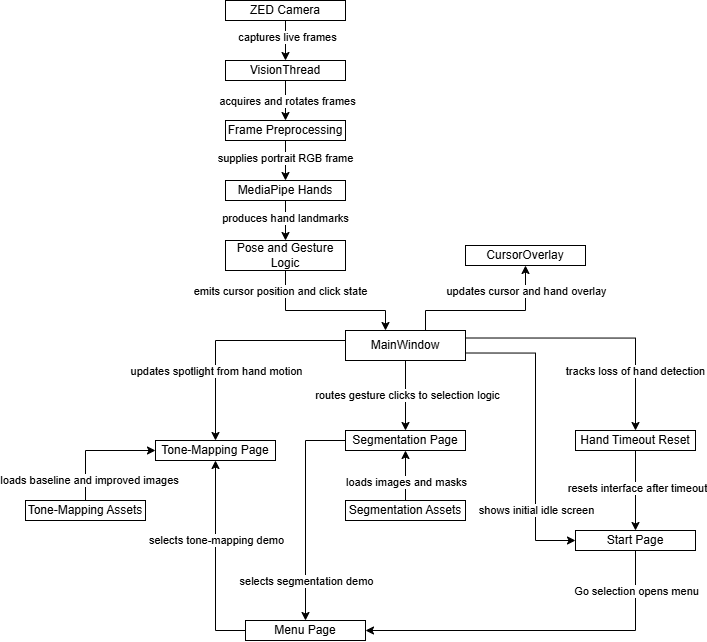
\includegraphics[width=0.95\textwidth]{4006_software_report-demo_diagram.drawio.png}
\caption{Architecture of the interactive demo, showing the live hand-tracking pipeline, central window controller, and gesture-driven demo pages.}
\label{fig:interactive-demo-architecture}
\end{figure}

\subsection{Data Model(s), Including In-Memory Structures and Persistent Storage}

The main runtime inputs are frames from the ZED camera
together with locally stored microscopy images, masks, and tone-mapped image
pairs. In memory, these are represented as image buffers, hand-tracking
outputs, cursor and gesture state, connected-component overlays for the
segmentation demonstration, and fixed baseline or improved image pairs for the
tone-mapping demonstration. Persistent storage is file-based rather than
database-based.

\medskip

This data model was chosen because it matched the role of the demo as a
live presentation tool rather than as a general-purpose software platform. The
application needed to combine real-time camera input with a small set of
prepared assets and transform them into responsive visual behaviour with as
little overhead as possible. A lightweight in-memory representation was
therefore appropriate, while file-based storage was sufficient because the demo
uses a fixed asset set and does not need complex persistence, remote access, or
long-term state management.

\medskip

Alternative designs were possible. For example, the prepared assets could have
been managed through a more elaborate asset-management layer or a database-backed
store. The visual outputs could also have been generated dynamically
rather than being read from prepared files. These approaches were not adopted
because they would have introduced additional complexity without clear benefit
for a demo whose purpose was to present fixed prepared
outputs through gesture-based interaction. The simpler file-based and
in-memory approach was therefore the more suitable design for this software.


\subsection{Significant Methods, Functions, or Other Lower-Level Elements}

The most significant lower-level elements in this demonstrator are the helper
functions and classes that convert hand landmarks into usable interaction
behaviour. Functions such as \texttt{palm\_center}, \texttt{palm\_width},
\texttt{tip\_mcp\_norm}, and \texttt{is\_fist} in
\path{mp_handpose_demo/hand_18.py} are important because they define how the
software derives cursor position, hand scale, and click-like gesture state
from the tracked hand landmarks.

\medskip

The \texttt{VisionThread} class,
performs live camera acquisition, frame preprocessing, MediaPipe hand
tracking, and click debouncing before emitting pose updates to the rest of the
application. forming the main runtime bridge
between raw camera input and the higher-level gesture-driven behaviour seen by
the user.

\medskip

The presentation behaviour of the demonstrator is implemented mainly through
\texttt{CursorOverlay}, \texttt{SegmentationDemoWidget},
\texttt{MultiMaskSegmentationWidget}, and \texttt{ToneMappingDemoWidget}.
These classes are significant because they implement the visible behaviour of
the two demonstrations: drawing the live overlay, resolving clicked
segmentation regions, revealing RNvU masks, and displaying the hand-controlled
tone-mapping spotlight. The \texttt{MainWindow} class coordinates these components and routes the
gesture-derived events that connect tracking input to page behaviour.


\subsection{Important Errors and Their Conditions}

The software may
fail to start correctly if the ZED camera is not connected, cannot be opened,
or is otherwise unavailable at runtime.
Parts of
the demonstrator may fail or display incomplete behaviour if required images or
mask files are missing, unreadable, or empty. Because the implementation uses
relative asset paths, the software also depends on being launched from the
expected working directory so that those paths resolve correctly.
Even
when the application starts successfully, behaviour may degrade if the user's
hand is not tracked reliably, if gesture detection is unstable, or if tracking
is lost during use. Under these conditions, cursor motion may become unstable,
intended selections may not register correctly, or the interface may return to
the start screen after the configured timeout. 

\subsection{User Interface Design}

The interaction logic is implemented explicitly rather than through a generic
gesture library. The cursor position is derived from the mean position of a
small set of palm-related landmarks, mirrored horizontally to match user
expectation, and then smoothed before being displayed so that motion appears
stable rather than jittery. A fist is detected by comparing fingertip-to-base
distances against palm width, and clicks are debounced so that one closing
motion does not trigger repeated activations. If no hand is detected for a
short timeout period, the interface automatically returns to the start screen,
which helps recover from tracking loss during live use. In practical terms,
this gives the demo two forms of interaction: continuous hand motion is
used to control cursor-like behaviour, while discrete fist closures are used as
selection events for navigation and page-specific actions.

\medskip

The first demonstration is event-driven. It presents microscopy imagery
together with precomputed segmentation data, and a user selection event
determines which prepared overlay is revealed. In one mode, a binary mask is
converted into connected components and the selected component is highlighted
when the user clicks on the image. In another mode, multiple precomputed RNvU
retina masks are loaded and the mask covering the selected pixel is revealed.

\medskip

The second demonstration is continuous rather than event-driven. It presents
tone-mapping results using paired images: a baseline image is shown across the
whole display, while an improved image is revealed only inside a
hand-controlled spotlight. The spotlight position follows the
gesture-controlled cursor and its radius scales with palm width, so hand motion
acts as a live control input rather than as a sequence of clicks. In both
demonstrations, the software does not run segmentation or tone-mapping models
live. It instead provides an interaction layer for exploring prepared outputs
visually.

\subsection{Quality Assurance Steps}

\subsubsection{Version Control and Versioning}

Development of the demonstrator was managed through Git-based version control.
This made it possible to track changes to the application logic,
documentation, and bundled assets while the interaction model and presentation
flow were still being refined. 

\subsubsection{Code Style and Convention}

Although the demonstrator is implemented largely in a single file, a consistent
internal structure was used to keep the code understandable. Configuration
constants are grouped near the top of the file, helper functions implement the
gesture calculations, dedicated widget classes encapsulate the different demo
views, and the \texttt{MainWindow} class coordinates page flow and interaction
state. Descriptive naming and lightweight inline documentation were used to
keep the behaviour clear during development.

\end{document}
